\begin{center}
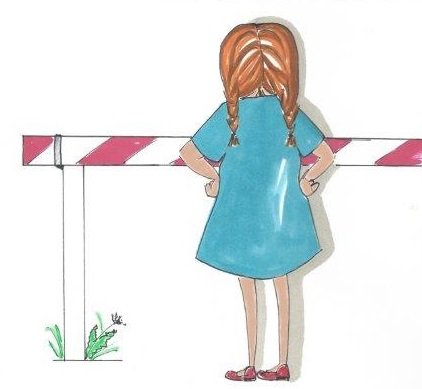
\includegraphics[width=0.6\textwidth]{content/3/chapter6/images/18.png}\\
Cippi waits at the barrier
\end{center}

Latches and barriers are coordination types that enable some threads to block until a counter becomes zero. In C++20 we get latches and barriers in two variations: std::latch and std::barrier. Concurrent invocations of the member functions of a std::latch or a std::barrier produce no data race.

First, there are two questions:

\begin{enumerate}
\item 
What is the difference between these two mechanisms to coordinate threads? You can use a std::latch only once, but you can use a std::barrier more than once. A std::latch is useful for managing one task by multiple threads. A std::barrier helps managing repeated tasks by multiple threads. Additionally, a std::barrier enables you to execute a function in the so-called completion step. The completion step is the state when the counter becomes zero.

\item 
What use cases do latches and barriers support that cannot be done in C++11 and C++14 with futures, threads, or condition variables combined with locks? Latches and barriers address no new use cases, but they are a lot easier to use. They are also more performant because they often use a \href{https://en.wikipedia.org/wiki/Non-blocking_algorithm}{lock-free} mechanism internally.
\end{enumerate}

\subsubsubsection{6.4.1\hspace{0.2cm} std::latch}

Now, let us have a closer look at the interface of a std::latch.

\begin{center}
Member functions of a std::latch lat
\end{center}

\begin{table}[H]
\centering
\begin{tabular}{ll}
\textbf{Member function} & \textbf{Description}          \\ \hline
lat.count\_down(upd = 1)       & Atomically decrements the counter by upd without blocking the caller.  \\
lat.try\_wait()          & Returns true if counter == 0. \\
lat.wait()                     & Returns immediately if counter == 0. If not blocks until counter == 0. \\
lat.arrive\_and\_wait(upd = 1) & Equivalent to count\_down(upd); wait();.                              
\end{tabular}
\end{table}

The default value for upd is 1. When upd is greater than the counter or negative, the behavior is undefined. The call lat.try\_wait() never actually waits, as its name suggests.

The following program bossWorkers.cpp uses two std::latch to build a boss-workers workflow. I synchronized the output to std::cout using the function synchronizedOut (line 13). This synchronization makes it easier to follow the workflow.

\hspace*{\fill} \\ %插入空行
\noindent
A boss-worker workflow using two std::latch
\begin{lstlisting}[style=styleCXX]
// bossWorkers.cpp

#include <iostream>
#include <mutex>
#include <latch>
#include <thread>

std::latch workDone(6);
std::latch goHome(1);

std::mutex coutMutex;

void synchronizedOut(const std::string& s) {
	std::lock_guard<std::mutex> lo(coutMutex);
	std::cout << s;
}

class Worker {
public:
	Worker(std::string n): name(n) { }
	
	void operator() (){
		// notify the boss when work is done
		synchronizedOut(name + ": " + "Work done!\n");
		workDone.count_down();
		
		// waiting before going home
		goHome.wait();
		synchronizedOut(name + ": " + "Good bye!\n");
	}
private:
	std::string name;
};

int main() {

	std::cout << '\n';
	
	std::cout << "BOSS: START WORKING! " << '\n';
	
	Worker herb(" Herb");
	std::thread herbWork(herb);
	
	Worker scott(" Scott");
	std::thread scottWork(scott);
	
	Worker bjarne(" Bjarne");
	std::thread bjarneWork(bjarne);
	
	Worker andrei(" Andrei");
	std::thread andreiWork(andrei);
	
	Worker andrew(" Andrew");
	std::thread andrewWork(andrew);
	
	Worker david(" David");
	std::thread davidWork(david);
	
	workDone.wait();
	
	std::cout << '\n';
	
	goHome.count_down();
	
	std::cout << "BOSS: GO HOME!" << '\n';
	
	herbWork.join();
	scottWork.join();
	bjarneWork.join();
	andreiWork.join();
	andrewWork.join();
	davidWork.join();

}
\end{lstlisting}

The idea of the workflow is straightforward. The six workers herb, scott, bjarne, andrei, andrew, and david (lines 41 - 57) have to fulfill their job. When each has finished his job, it counts down the std::latch workDone (line 25). The boss (main-thread) is blocked in line 59 until the counter becomes 0. When the counter is 0, the boss uses the second std::latch goHome to signal its workers to go home. In this case, the initial counter is 1 (line 9). The call goHome.wait() blocks until the counter becomes 0.

\begin{center}
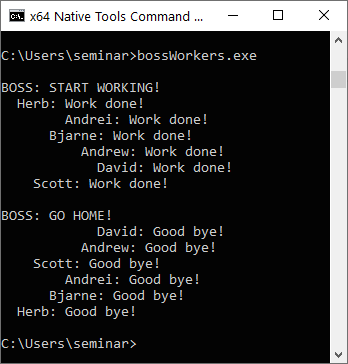
\includegraphics[width=0.6\textwidth]{content/3/chapter6/images/19.png}\\
A boss-worker workflow using two std::latch
\end{center}

When you think about this workflow, you may notice that it can be performed without a boss. Here it is.

\hspace*{\fill} \\ %插入空行
\noindent
A worker’s workflow using a std::latch
\begin{lstlisting}[style=styleCXX]
// workers.cpp

#include <iostream>
#include <barrier>
#include <mutex>
#include <thread>

std::latch workDone(6);
std::mutex coutMutex;

void synchronizedOut(const std::string& s) {
	std::lock_guard<std::mutex> lo(coutMutex);
	std::cout << s;
}

class Worker {
public:
	Worker(std::string n): name(n) { }

	void operator() () {
		synchronizedOut(name + ": " + "Work done!\n");
		workDone.arrive_and_wait(); // wait until all work is done
		synchronizedOut(name + ": " + "See you tomorrow!\n");
	}
private:
	std::string name;
};

int main() {

	std::cout << '\n';
	
	Worker herb(" Herb");
	std::thread herbWork(herb);
	
	Worker scott(" Scott");
	std::thread scottWork(scott);
	
	Worker bjarne(" Bjarne");
	std::thread bjarneWork(bjarne);
	
	Worker andrei(" Andrei");
	std::thread andreiWork(andrei);
	
	Worker andrew(" Andrew");
	std::thread andrewWork(andrew);
	
	Worker david(" David");
	std::thread davidWork(david);
	
	herbWork.join();
	scottWork.join();
	bjarneWork.join();
	andreiWork.join();
	andrewWork.join();
	davidWork.join();

}
\end{lstlisting}

There is not much to add to this simplified workflow. The call wordDone.arrive\_and\_wait() (line 22) is equivalent to the calls count\_down(upd); wait();. This means the workers coordinate themselves and the boss is no longer necessary, as was the case in the previous program bossWorkers.cpp.

\begin{center}
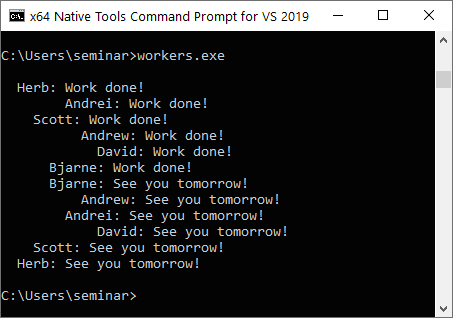
\includegraphics[width=0.6\textwidth]{content/3/chapter6/images/20.png}\\
A workers workflow using a std::latch
\end{center}

A std::barrier is similar to a std::latch.

\subsubsubsection{6.4.2\hspace{0.2cm} std::barrier}

There are two differences between a std::latch and a std::barrier. First, you can use a std::barrier more than once, and second, you can set the counter for the next step (iteration). Immediately after the counter becomes zero, the so-called completion step starts. In this completion step, a callable is invoked. The std::barrier gets its callable in its constructor.

The completion step performs the following steps:

\begin{enumerate}
\item 
All threads are blocked.

\item 
An arbitrary thread is unblocked and executes the callable.

\item 
If the completion step is done, all threads are unblocked.
\end{enumerate}

\begin{center}
Member functions of a std::barrier bar
\end{center}

\begin{table}[H]
\centering
\begin{tabular}{ll}
Member function         & Description                                   \\ \hline
bar.arrive(upd)         & Atomically decrements counter by upd.         \\
bar.wait()              & Blocks at the synchronization point until the completion step is done.  \\
bar.arrive\_and\_wait() & Equivalent to wait(arrive())                  \\
bar.arrive\_and\_drop() & Decrements the counter for the current and the subsequent phase by one. \\
std::barrier::max       & Maximum value supported by the implementation
\end{tabular}
\end{table}

The call bar.arrive\_and\_drop() means essentially that the counter is decremented by one for the next phase. The program fullTimePartTimeWorkers.cpp halves the number of workers in the second phase.

\hspace*{\fill} \\ %插入空行
\noindent
Full-time and part-time workers
\begin{lstlisting}[style=styleCXX]
// fullTimePartTimeWorkers.cpp

#include <iostream>
#include <barrier>
#include <mutex>
#include <string>
#include <thread>

std::barrier workDone(6);
std::mutex coutMutex;

void synchronizedOut(const std::string& s) {
	std::lock_guard<std::mutex> lo(coutMutex);
	std::cout << s;
}

class FullTimeWorker {
public:
	FullTimeWorker(std::string n): name(n) { }
	
	void operator() () {
		synchronizedOut(name + ": " + "Morning work done!\n");
		workDone.arrive_and_wait(); // Wait until morning work is done
		synchronizedOut(name + ": " + "Afternoon work done!\n");
		workDone.arrive_and_wait(); // Wait until afternoon work is done

	}
private:
	std::string name;
};

class PartTimeWorker {
public:
	PartTimeWorker(std::string n): name(n) { }

	void operator() () {
		synchronizedOut(name + ": " + "Morning work done!\n");
		workDone.arrive_and_drop(); // Wait until morning work is done
	}
private:
	std::string name;
};

int main() {

	std::cout << '\n';
	
	FullTimeWorker herb(" Herb");
	std::thread herbWork(herb);
	
	FullTimeWorker scott(" Scott");
	std::thread scottWork(scott);
	
	FullTimeWorker bjarne(" Bjarne");
	std::thread bjarneWork(bjarne);
	PartTimeWorker andrei(" Andrei");
	std::thread andreiWork(andrei);
	
	PartTimeWorker andrew(" Andrew");
	std::thread andrewWork(andrew);
	
	PartTimeWorker david(" David");
	std::thread davidWork(david);
	
	herbWork.join();
	scottWork.join();
	bjarneWork.join();
	andreiWork.join();
	andrewWork.join();
	davidWork.join();

}
\end{lstlisting}

This workflow consists of two kinds of workers: full-time workers (line 17) and part-time workers (line 32). The part-time worker works in the morning, the full-time worker in the morning and the afternoon. Consequently, the full-time workers call workDone.arrive\_and\_wait() (lines 23 and 25) two times. On the contrary, the part-time workers call workDone.arrive\_and\_drop() (line 38) only once. This workDone.arrive\_and\_drop() call causes the part-time worker to skip the afternoon work. Accordingly, the counter has in the first phase (morning) the value 6, and in the second phase (afternoon) the value 3.

\begin{center}
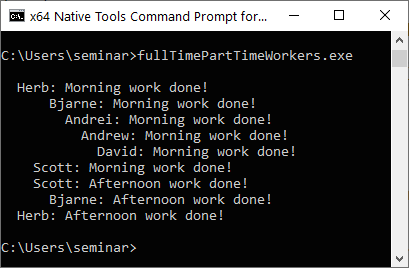
\includegraphics[width=0.6\textwidth]{content/3/chapter6/images/21.png}\\
Full-time and part-time workers
\end{center}

\begin{tcolorbox}[breakable,enhanced jigsaw,colback=mygreen!5!white,colframe=mygreen!75!black,title={Distilled Information}]
	
\begin{itemize}
\item 
Latches and barriers are coordination types that enable some threads to block until a counter becomes zero. You can use a std::latch only once, but you can use a std::barrier more than once.

\item 
A std::latch is useful for managing one task by multiple threads; a std::barrier helps manage repeated tasks by multiple threads.
\end{itemize}
	
\end{tcolorbox}

\newpage














